\chapter{Results} \label{ch:results}

%----------------------------------------
% EXPERIMENTS
%----------------------------------------
\section{Experiments}

	The experiments were run using Cessna 172S flight data produced by students at the University of North Dakota during the month of September 2015.  Student flight data is ideal for unstable analysis testing as it contains very noisy data, which provides a diverse array of flying patterns.  A random sample of 100 flights was chosen for the experiments.
        
    First, the application was run against the 100 flights to obtain the automated analysis results.  The same 100 flights were then manually analyzed in order to get human results, which could be compared to the automated results then determine the accuracy of the application.  The test of the 100 flights was also run ten times each with the single-process version and the multi-process version as previously described.  This was done in order to compare and contrast the performance of the separate versions.


%----------------------------------------
% QUALITY
%----------------------------------------
\section{Quality}

	The manual validation was performed using a combination of tools available on the NGAFID website:  the Cesium flight reanimation tool and the Keyhole Markup Language (KML) generator to visualize the flight path on Google Earth~\cite{nolan2014keyhole} (see \Cref{fig:kml_example}).
    
    \begin{figure}
    	\centering
        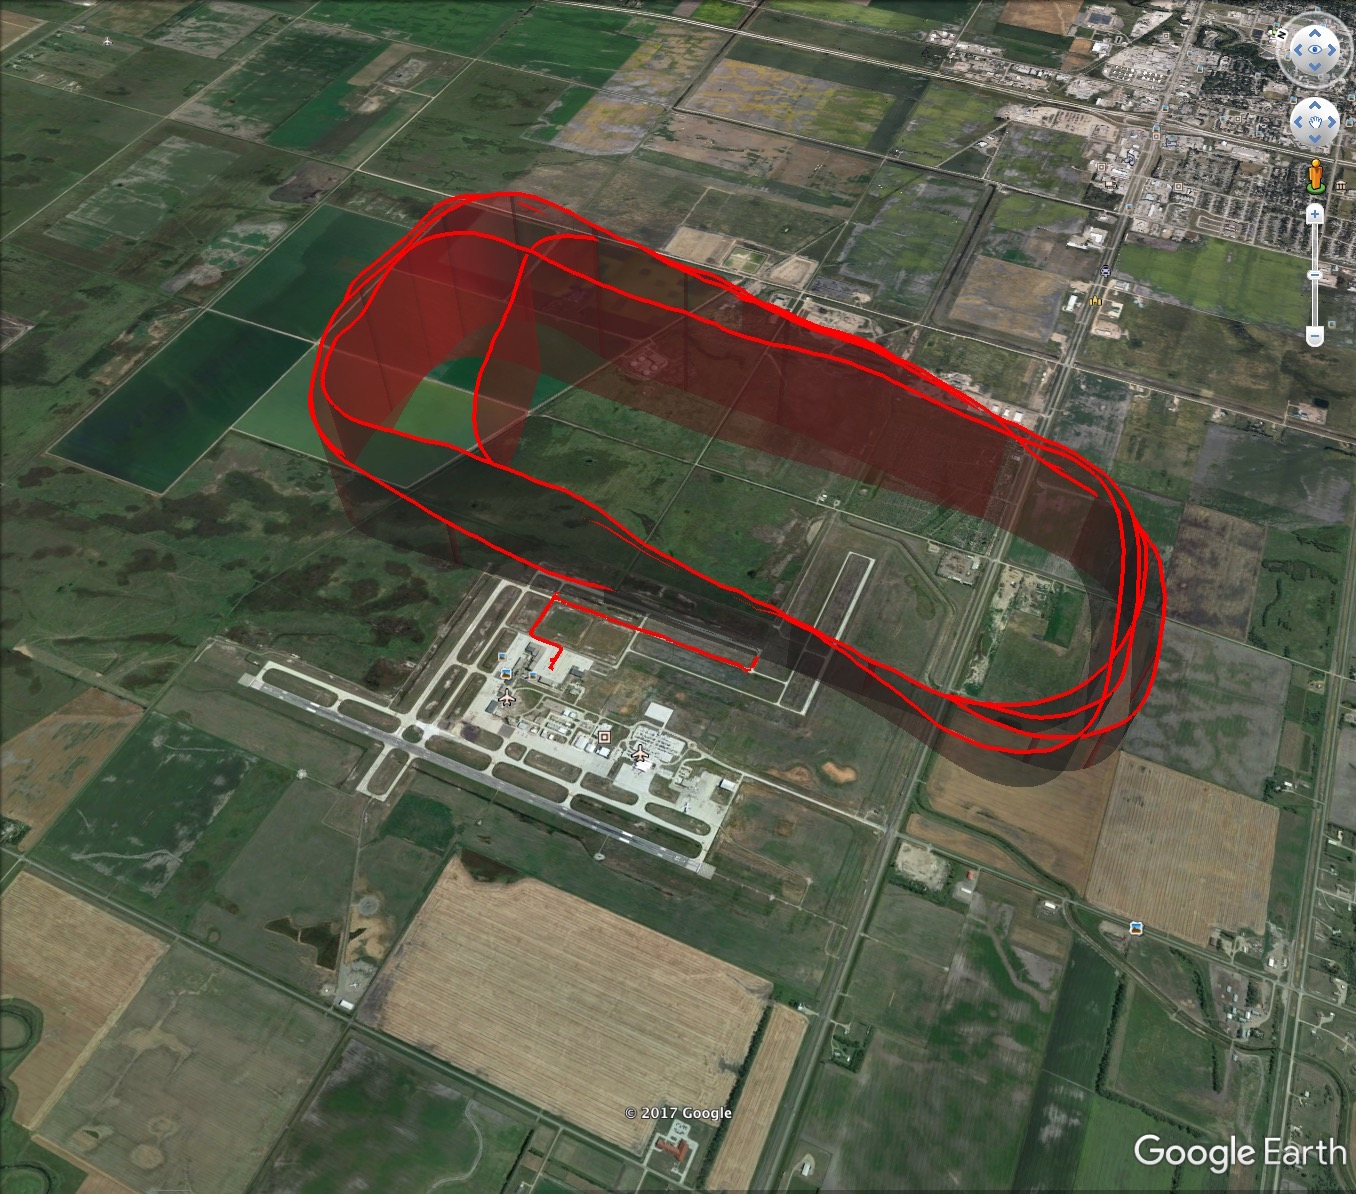
\includegraphics[width=\linewidth]{img/kml_example}
        \caption{Example of using a KML file to visualize a flight path in Google Earth.  This flight visualization is an example of a student flight that has multiple final approach phases.}
        \label{fig:kml_example}
    \end{figure}
    
    
    %----------
    % APPROACH
    %----------
    \subsection{Approach}
    
        The \toolname\ generated a total of 377 approaches for the 100 flights that were tested. As seen in \Cref{fig:kml_example}, student flights typically consist of multiple approaches as this is something that needs to be practiced.  Out of the total; there are 370 (98.14\%) true positives, five (1.33\%) false positives, and two (0.53\%) false negatives.  These results can also be found in \Cref{fig:validation_results}.  In the context of this application, a true positive is a case where the tool correctly indicates that an approach is occurring during a specified time frame.  A false positive occurs when the tool indicates that an approach is occurring but is not in reality.  Typically, a false positive occurs when the flight data has invalid values for about the first ten rows, which then throws off the beginning of the algorithms.  This happens infrequently, but could be accounted for in a future work by sanitizing the data before analysis.  A false negative is the exact opposite where the tool indicates that an approach is not occurring but it is in reality.  Typically, a false negative occurs when the approached airport's geological data is not contained within the database.  These types of occurrences should stop once the airports database is expanded with more entries.  Lastly, the tool misclassified the approached runway 13 times (3.45\%).  A runway is misclassified when the difference between the aircraft and runway headings is greater than $20^\circ$.  This occurs during the runway detection portion of the approach analysis algorithm, and the algorithm either returns a \emph{null} runway or an incorrect runway due to the large heading difference.

        In this same context, it is difficult to quantify the number of true negatives since these would be cases where the tool correctly indicates that an approach is not occurring.  The difficulty lies in how to define a single occurrence.  Should a single true negative be counted for every second the tool indicates that an approach is not occurring?  If so, then this would create a numerous amount of true negatives and would dilute the percentages of the other statistics, which are more important in this application.

        The validation results demonstrate that the \toolname\ is exceptionally accurate in its ability to appropriately detect and classify most approaches in a flight.

        \begin{figure}
            \centering
            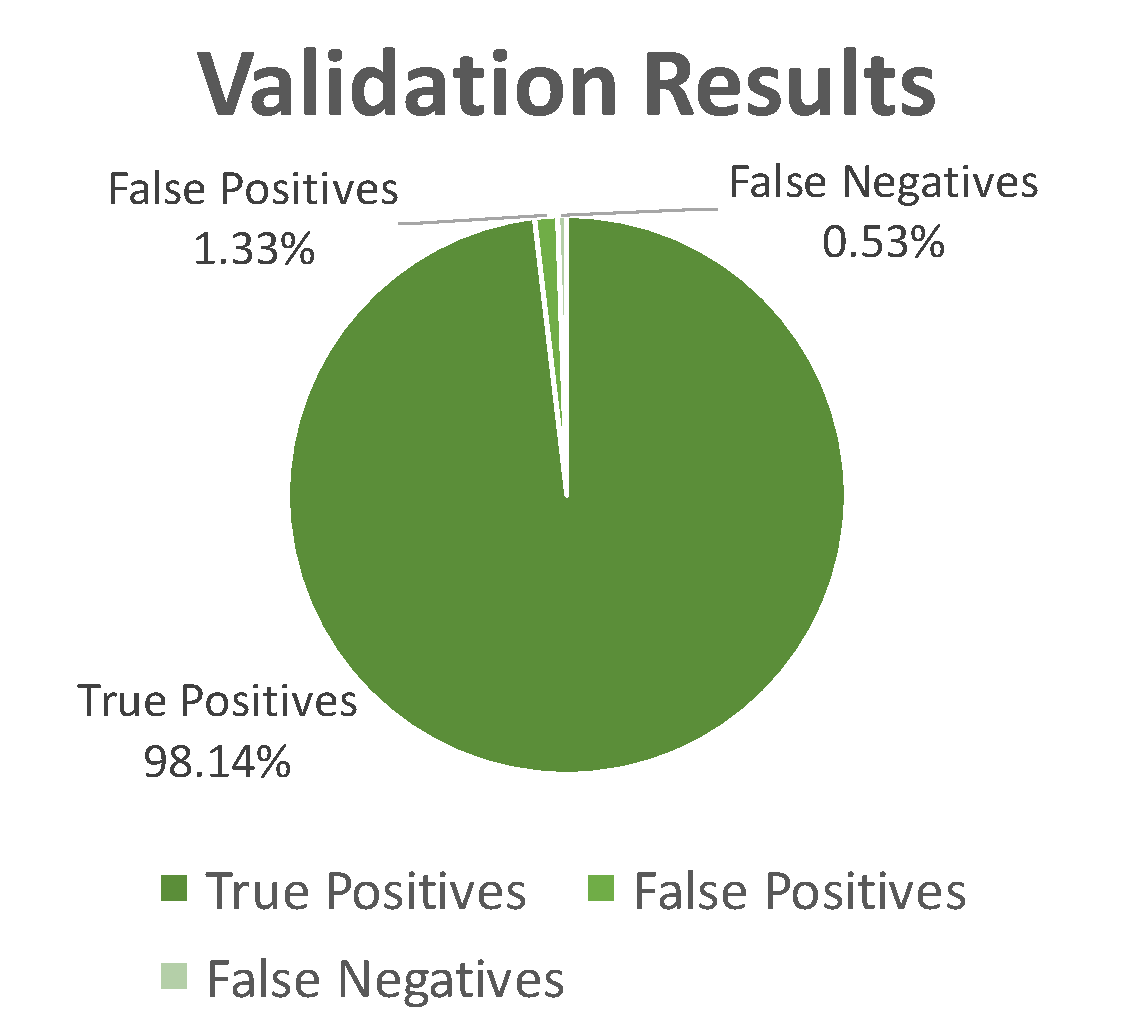
\includegraphics[width=0.5\linewidth]{img/validation_results}
            \caption{Pie chart showing the manual validation results including true positives, false positives, and false negatives.}
            \label{fig:validation_results}
        \end{figure}
        
        
    %----------
    % TAKEOFF
    %----------
    \subsection{Takeoff}
    
    	\note{Put in defense for why I did not do manual validation of Takeoffs.}
    
    
%----------------------------------------
% GRADING METRICS: DEFINE FROM PARAMETER FREQUENCIES
%----------------------------------------
\section{Grading Metrics:  Define From Parameter Frequencies}

	%----------
    % APPROACH
    %----------
    \subsection{Approach}
    
    	
        %----------
        % IAS
        %----------
    	\subsubsection{Indicated airspeed between 55 and 75 knots.}
        
            \begin{figure}
                \centering
                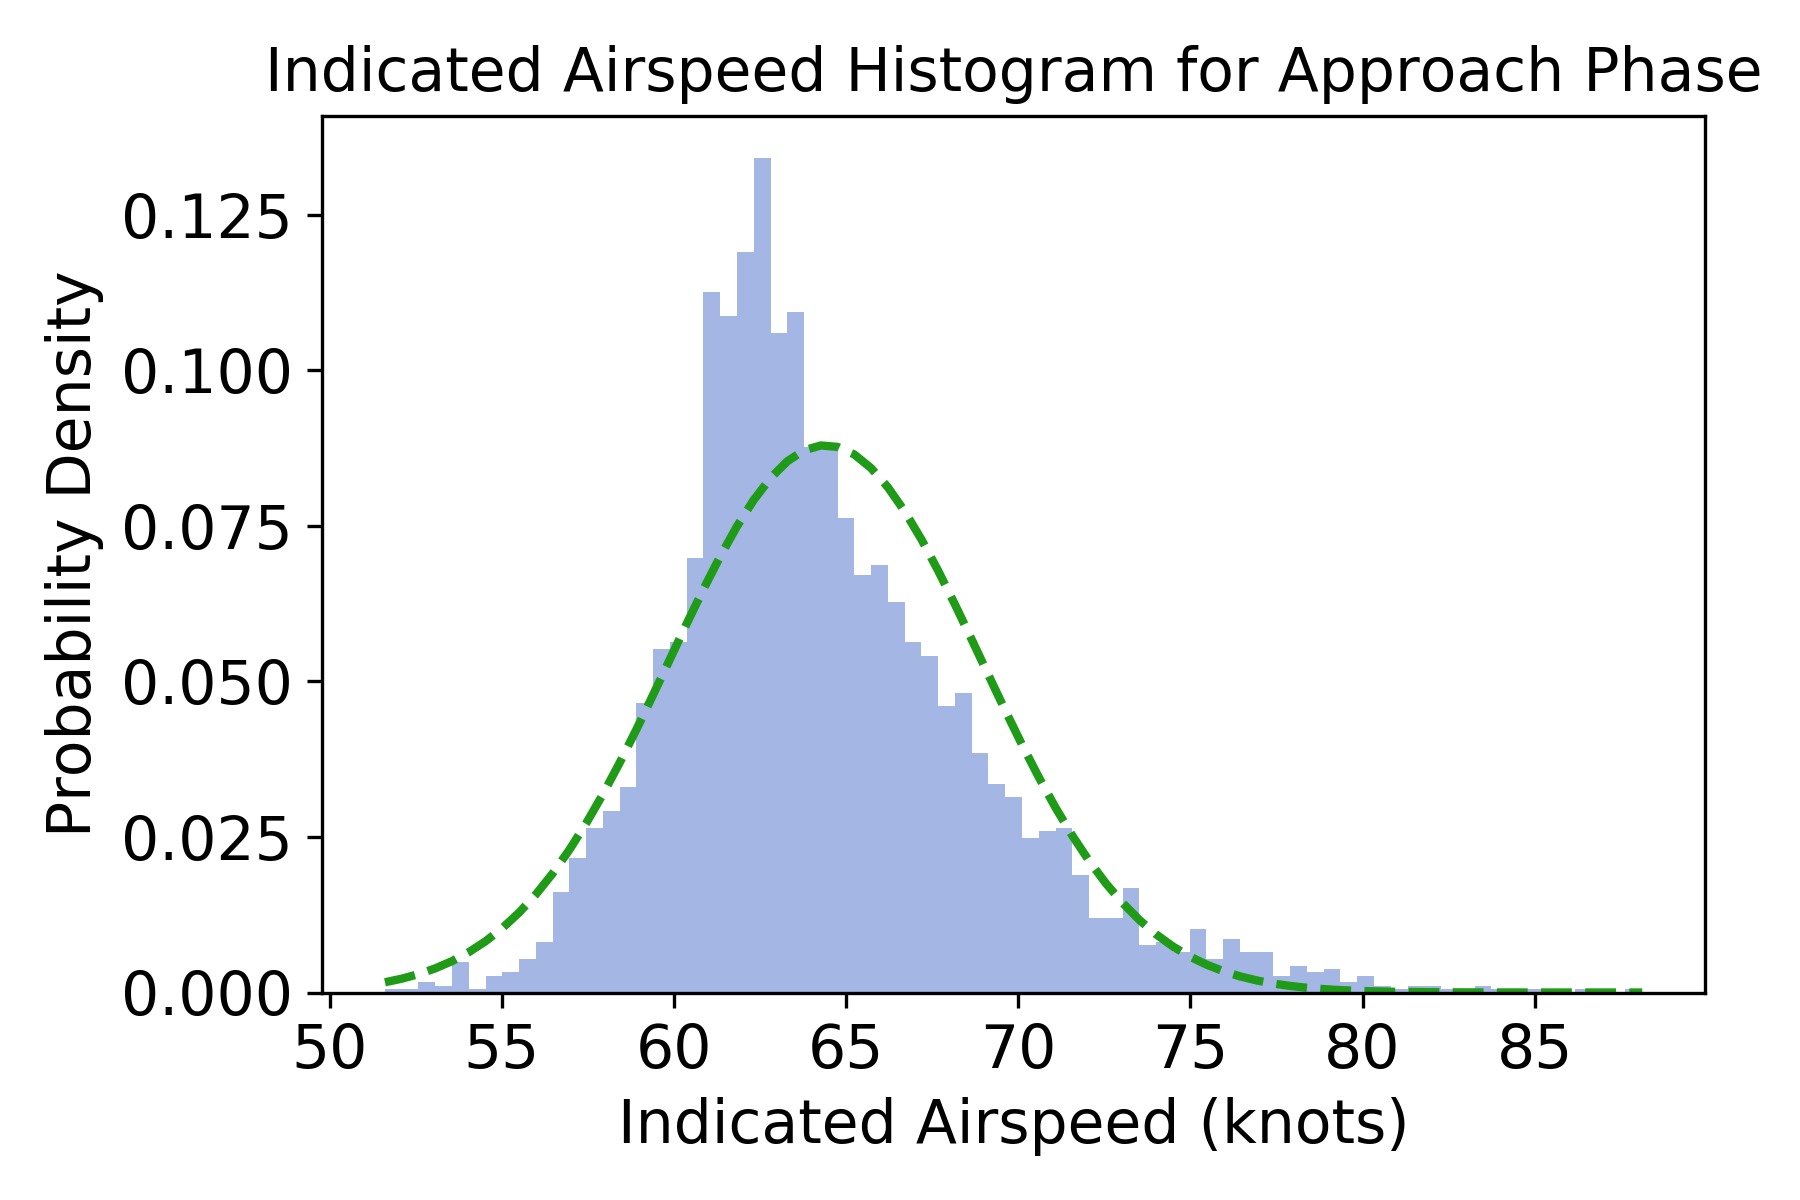
\includegraphics[width=\linewidth]{img/ias_hist}
                \caption{blah}
                \label{fig:approach_ias_hist}
            \end{figure}
        
        
        %----------
        % VSI
        %----------
    	\subsubsection{Vertical speed indicated greater than -1000 ft/min.}
        
            \begin{figure}
                \centering
                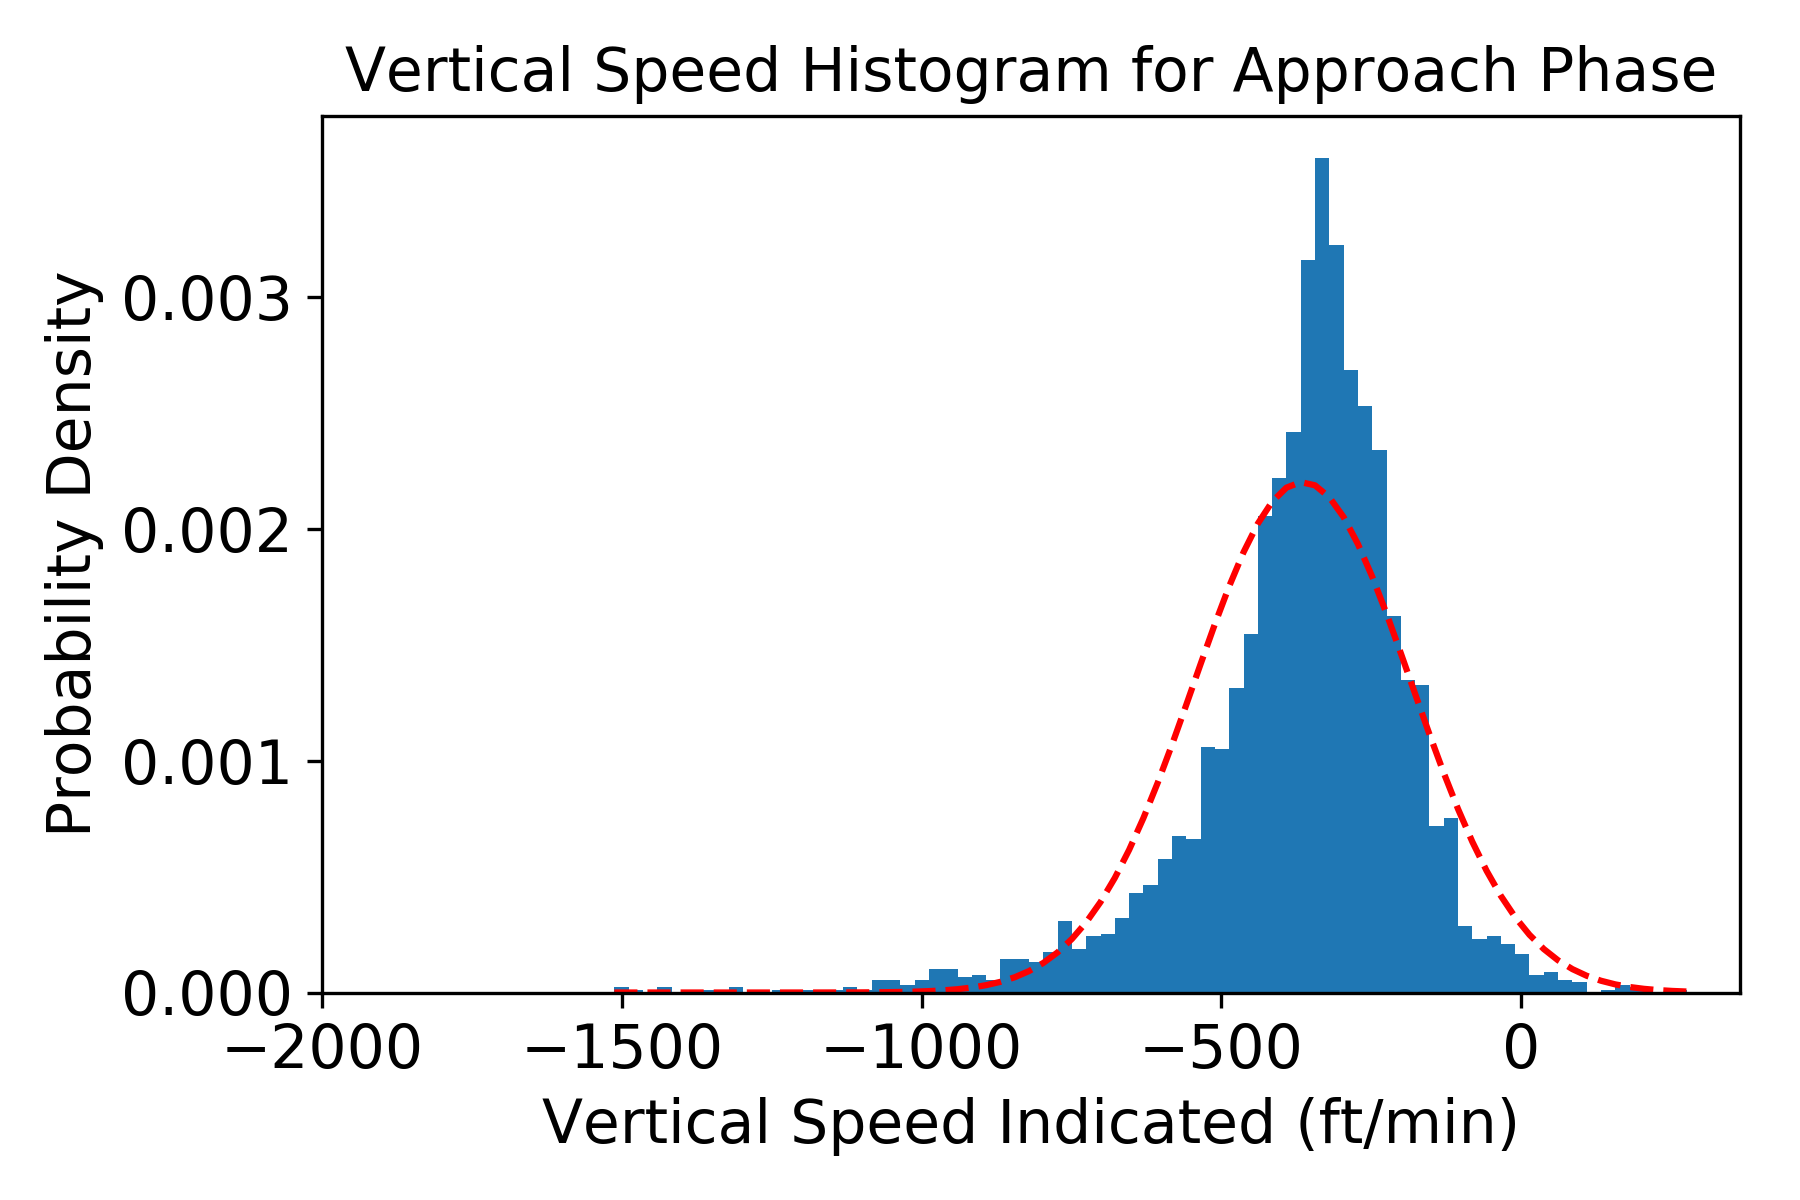
\includegraphics[width=\linewidth]{img/vsi_hist}
                \caption{blah}
                \label{fig:approach_vsi_hist}
            \end{figure}
        
        
        %----------
        % CROSS TRACK ERROR
        %----------
    	\subsubsection{Absolute cross track error less than 50 ft.}
        
            \begin{figure}
                \centering
                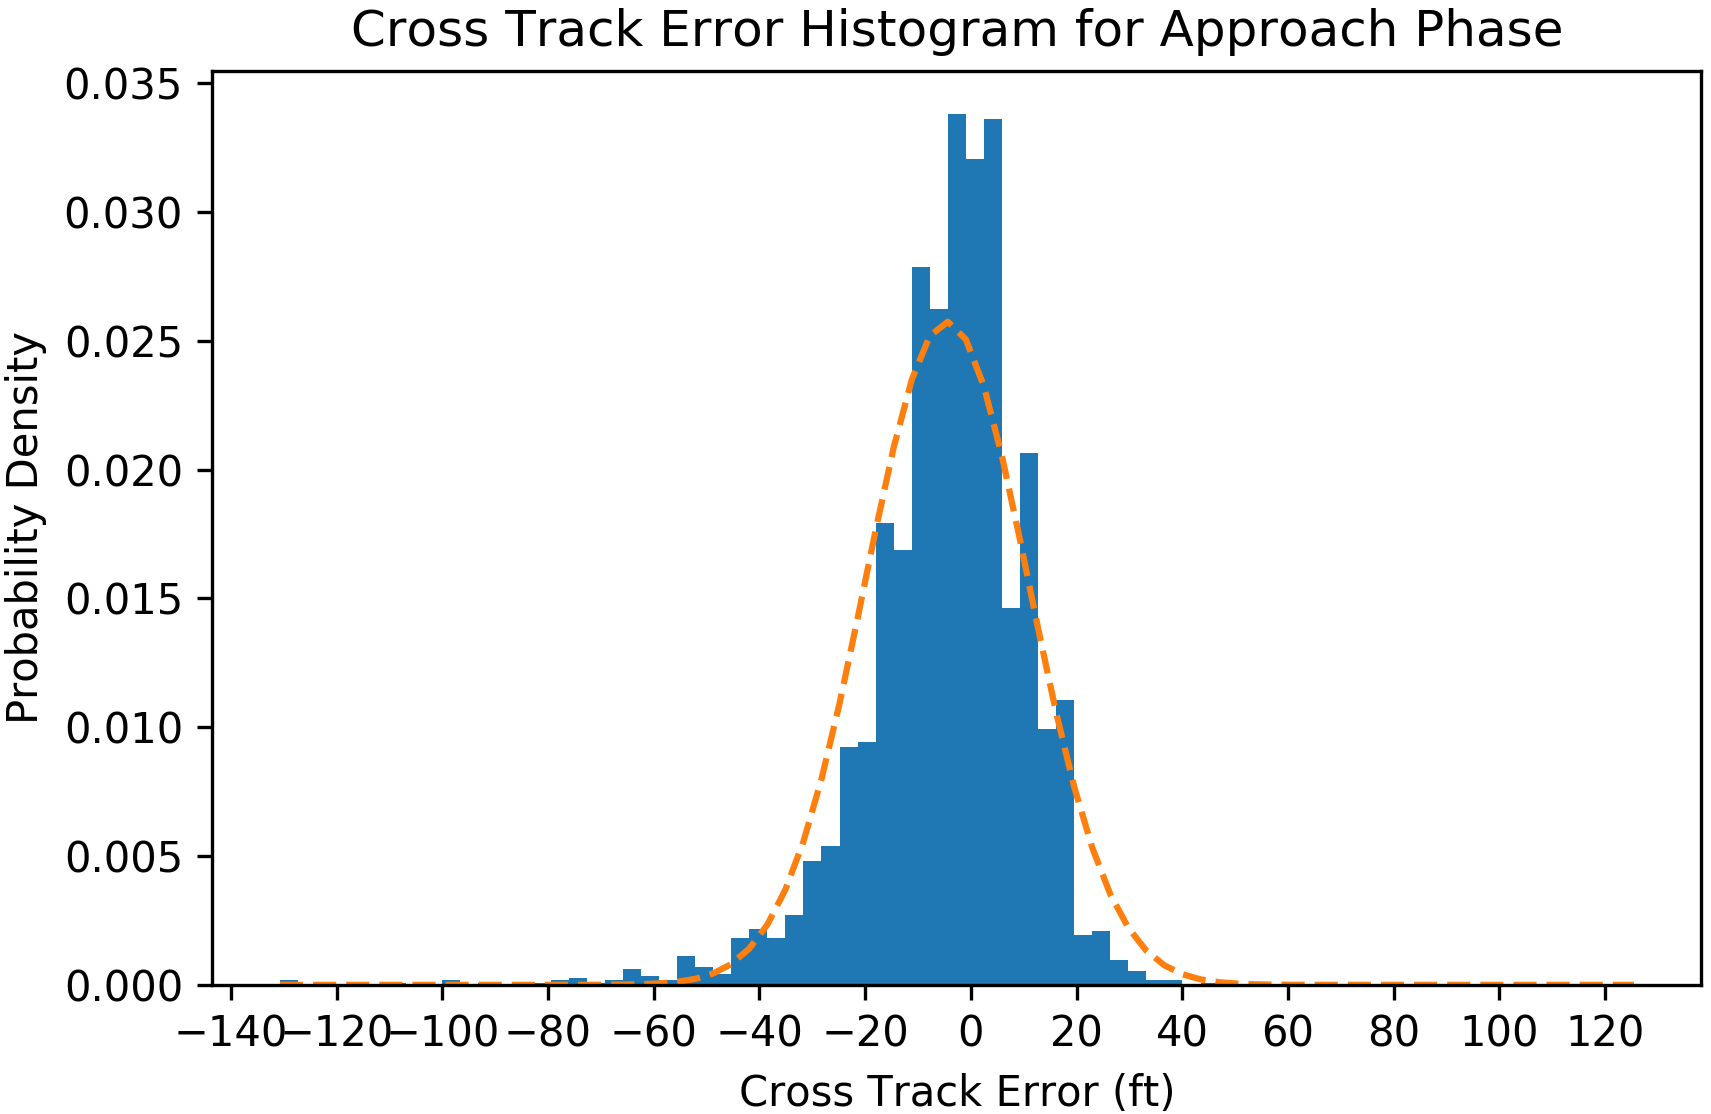
\includegraphics[width=\linewidth]{img/cross_track_hist}
                \caption{blah}
                \label{fig:approach_cross_track_hist}
            \end{figure}
            
            
        %----------
        % HEADING ERROR
        %----------
    	\subsubsection{Absolute heading error less than 10 degrees.}
        
            \begin{figure}
                \centering
                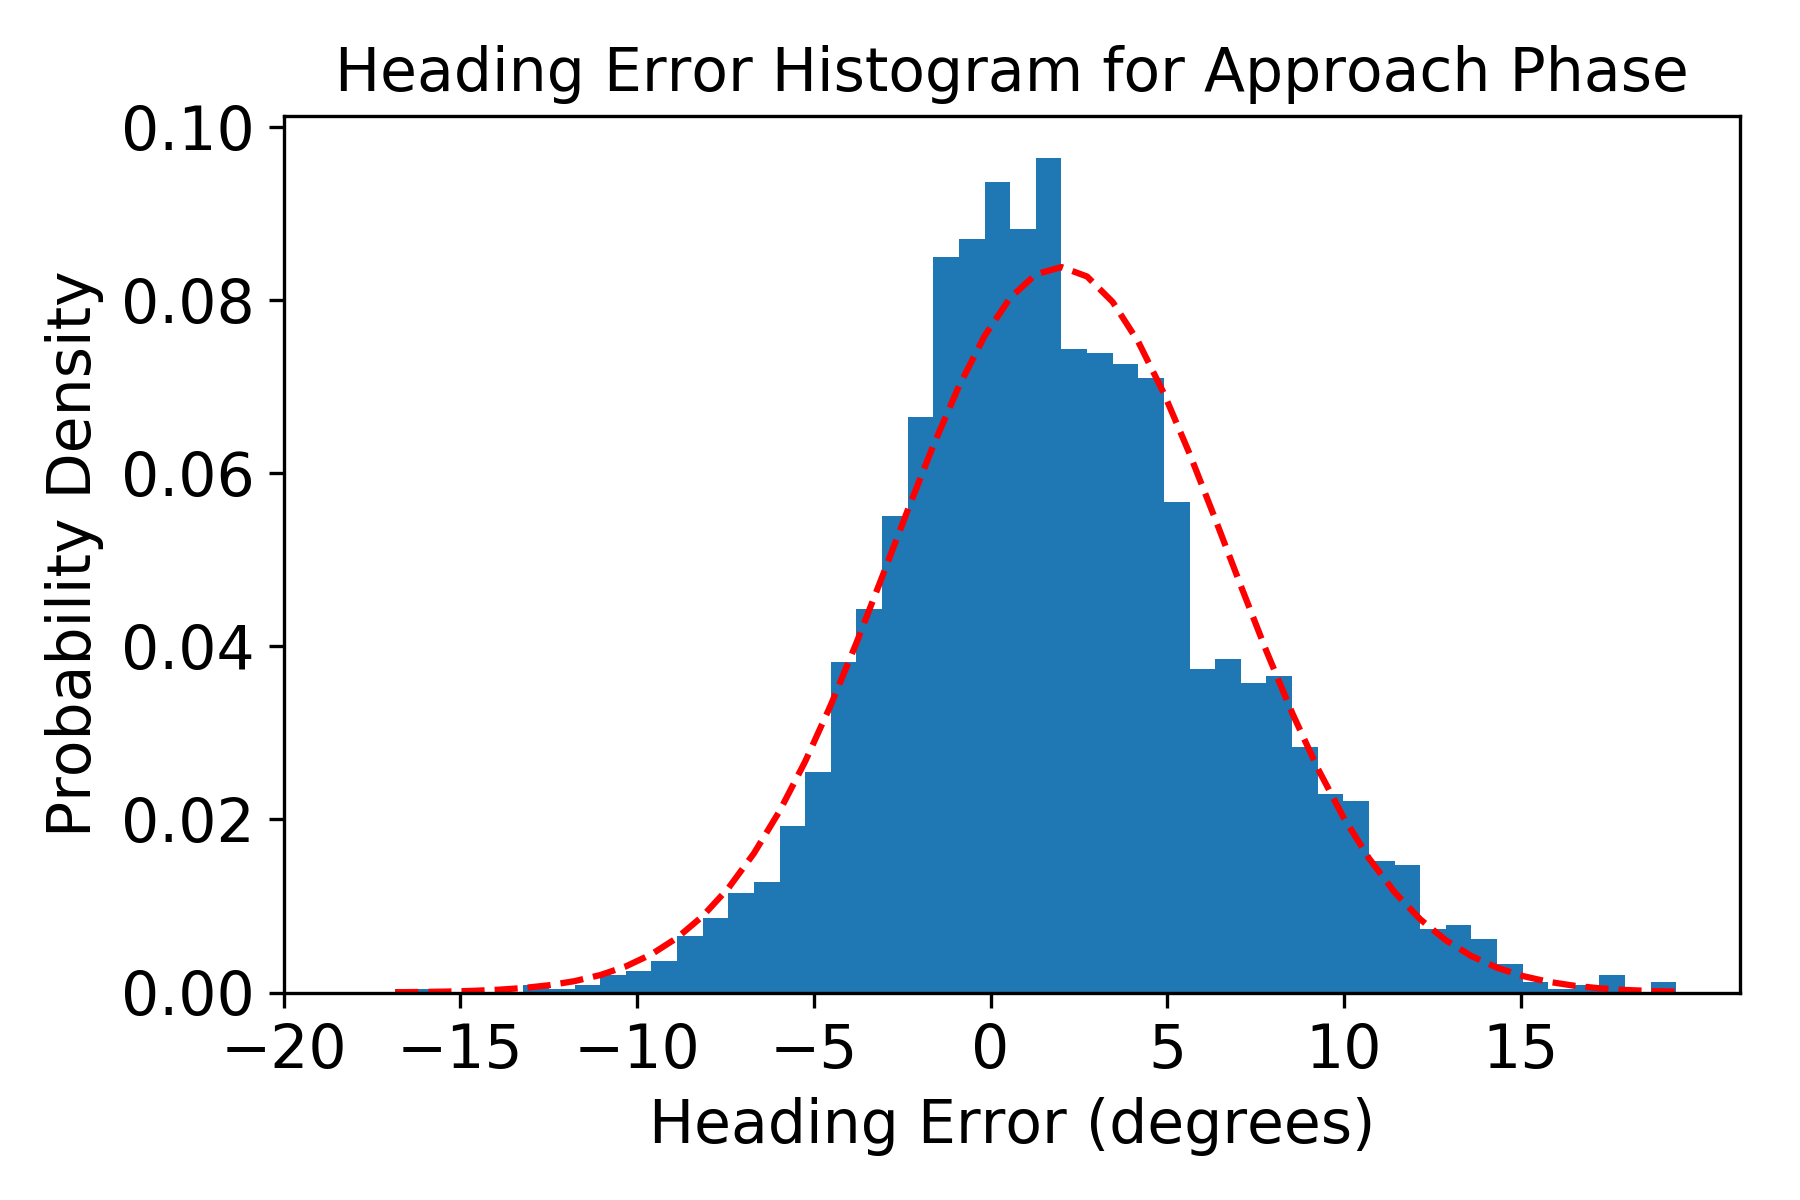
\includegraphics[width=\linewidth]{img/heading_hist}
                \caption{blah}
                \label{fig:approach_heading_hist}
            \end{figure}
    
    
%----------------------------------------
% GRADING METRICS: RESULTS
%----------------------------------------
\section{Grading Metrics:  Experiment Results}

	\note{Results found from using metrics on analysis results.}


%----------------------------------------
% PERFORMANCE
%----------------------------------------
\section{Performance}

	A secondary aspect of this research is to minimize the execution time so  the analysis only adds a minimal amount of time to a flight being imported into the NGAFID system.  The results of the benchmarking tests showed that the linearly executing application ran for an average of XXX.XXX seconds over the 100 randomly tested flights.  On the other hand, the parallel application ran for an average of XX.XXX seconds over the same flights.  This means the average per-flight execution times for the linear and parallel applications were X.XXX and X.XXX seconds, respectively.  As a result, the parallelized application had a XX.XXX\% speedup, which is fairly significant.  %A summary of the benchmarking tests and other relevant statistics are given in \Cref{tab:performance_results}.
    \note{Fill in timing results.}
    
    As further evidence, the parallel application was tested on a larger subset of flights to see if the average execution time remained stable, in which it was tested on 5,272 flights.  For this test, the parallel application was able to analyze the data and insert all the results into the database in XXXX.XXX seconds.  This gives a per-flight execution time of X.XXX seconds, which is slightly less than the average for 100 flights.  The reasoning behind this can most likely be attributed to the fact that spinning up the sub-processes creates a substantial overhead.  Thus, the longer the application is able to execute, the greater performance gain will be received.  This will, of course, start to show diminishing returns as with any other parallel computing application.
    
    
    \begin{table}[tb]
        \caption{\small{Performance of Linear v. Parallel Execution Times}}
        \vspace{3pt}
        \label{tab:performance_results}
        \centering
        \begin{tabular}{@{} >{\centering\arraybackslash} m{.23\linewidth} S[table-format=3.3] S[table-format=2.3] @{}}
            \hline\noalign{\smallskip}
            \bfseries Run & \bfseries Linear (sec) & \bfseries Parallel (sec) \\
            \noalign{\smallskip}
            \hline
            \noalign{\smallskip}
             1 & 591.935 & 57.295 \\ \hline
             2 & 576.774 & 60.282 \\ \hline
             3 & 586.009 & 57.830 \\ \hline
             4 & 597.643 & 62.489 \\ \hline
             5 & 591.170 & 57.578 \\ \hline
             6 & 585.834 & 62.702 \\ \hline
             7 & 593.711 & 65.064 \\ \hline
             8 & 587.177 & 66.167 \\ \hline
             9 & 586.059 & 58.108 \\ \hline
            10 & 590.012 & 56.501 \\ \hline
            \hline
            \bfseries Average           & 588.632 & 60.402   \\ \hline
            \bfseries Latency / flight  &   5.886 &  0.604   \\ \hline
            \bfseries Speedup           &         & 90.255\% \\ \hline
        \end{tabular}
    \end{table}
    
    
    
    